% Digital Logic Report Template
% Created: 2020-01-10, John Miller

%==========================================================
%=========== Document Setup  ==============================

% Formatting defined by class file
\documentclass[11pt]{article}

% ---- Document formatting ----
\usepackage[margin=1in]{geometry}	% Narrower margins
\usepackage{booktabs}				% Nice formatting of tables
\usepackage{graphicx}				% Ability to include graphics

%\setlength\parindent{0pt}	% Do not indent first line of paragraphs 
\usepackage[parfill]{parskip}		% Line space b/w paragraphs
%	parfill option prevents last line of pgrph from being fully justified

% Parskip package adds too much space around titles, fix with this
\RequirePackage{titlesec}
\titlespacing\section{0pt}{8pt plus 4pt minus 2pt}{3pt plus 2pt minus 2pt}
\titlespacing\subsection{0pt}{4pt plus 4pt minus 2pt}{-2pt plus 2pt minus 2pt}
\titlespacing\subsubsection{0pt}{2pt plus 4pt minus 2pt}{-6pt plus 2pt minus 2pt}

% ---- Hyperlinks ----
\usepackage[colorlinks=true,urlcolor=blue]{hyperref}	% For URL's. Automatically links internal references.

% ---- Code listings ----
\usepackage{listings} 					% Nice code layout and inclusion
\usepackage[usenames,dvipsnames]{xcolor}	% Colors (needs to be defined before using colors)

% Define custom colors for listings
\definecolor{listinggray}{gray}{0.98}		% Listings background color
\definecolor{rulegray}{gray}{0.7}			% Listings rule/frame color

% Style for Verilog
\lstdefinestyle{Verilog}{
	language=Verilog,					% Verilog
	backgroundcolor=\color{listinggray},	% light gray background
	rulecolor=\color{blue}, 			% blue frame lines
	frame=tb,							% lines above & below
	linewidth=\columnwidth, 			% set line width
	basicstyle=\small\ttfamily,	% basic font style that is used for the code	
	breaklines=true, 					% allow breaking across columns/pages
	tabsize=3,							% set tab size
	commentstyle=\color{gray},	% comments in italic 
	stringstyle=\upshape,				% strings are printed in normal font
	showspaces=false,					% don't underscore spaces
}

% How to use: \Verilog[listing_options]{file}
\newcommand{\Verilog}[2][]{%
	\lstinputlisting[style=Verilog,#1]{#2}
}


\usepackage[section]{placeins}

%======================================================
%=========== Body  ====================================
\begin{document}

\title{ELC 2137 Lab 7: Binary Coded Decimal}
\author{Aaron Mendoza}

\maketitle


\section*{Summary}

The purpose of this lab is to use the seven segment module I built in Lab 6 and use it to make the switches display a number in both decimal and hex. In order to do this, I had to implement the double-dabble algorithm into my Basys3 board by programming a file onto it from Vivado.

First, I began by understanding how the algorithm works. In order to convert hex values into BCD, the double-dabble algorithm is used. In this algorithm, the bits are shifted left. If the bits that are shifted left are greater than four, then you would add three to those bits and shift afterwards. This would convert the bits into BCD. 

Next, I had to write this module into SystemVerilog. I began by creating an add3 module. It would take a four-bit input and output another four bit number. If the input was greater than four, then I would add three to those bits. These modules are crucial in building the full double-dabble circuit because each circuit uses multiple add3 modules.

The second module I built was a 6-bit BCD converter module. It had an input of 6 bits; the three leftmost bits would read into the first add3 module with the leftmost bit of the add3 module being 0, and the output would cascade down into more add3 modules. The 6-bit BCD converter had only three add3 modules.

The third module I built was an 11-bit BCD converter module. It had an input of 11 bits, and followed the same pattern as the 6-bit module, but with fifteen add3 modules. 

\begin{figure}[ht]\centering
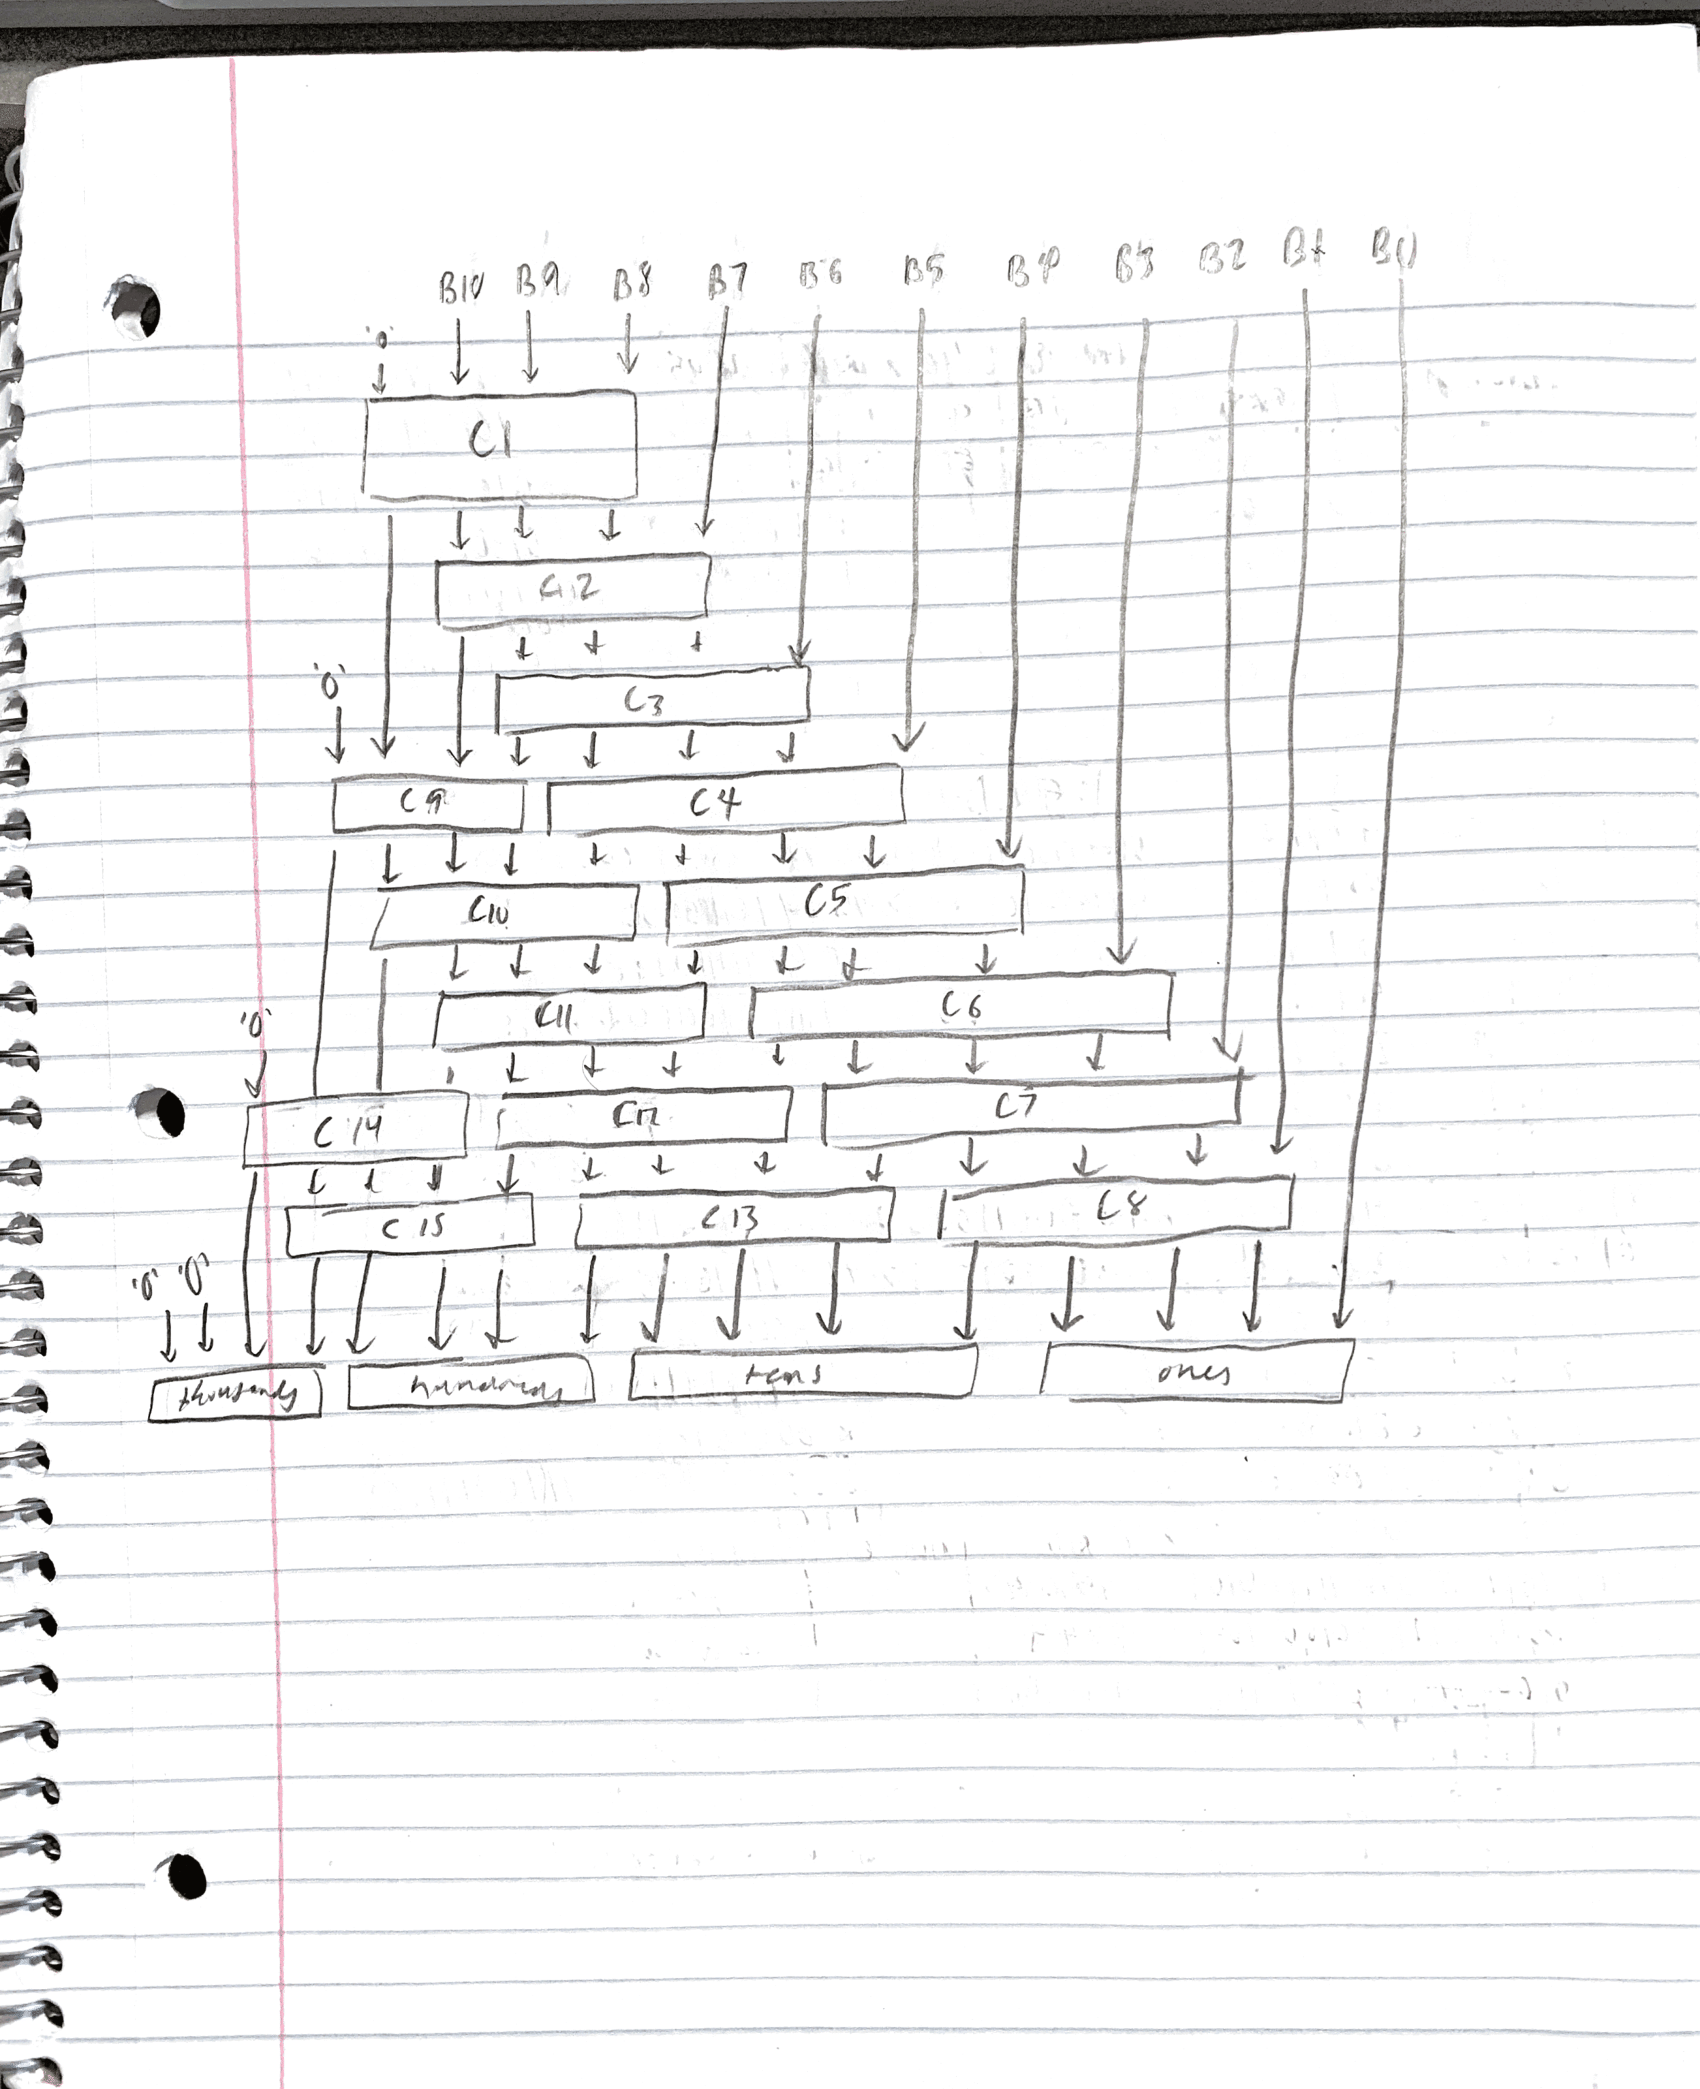
\includegraphics[width=0.5\textwidth]{eleven_BCD_diag}
\caption{This is an image of the 11-bit BCD converter circuit diagram.}
\label{fig:original_logo}
\end{figure}

The final module built combined the sseg module created in lab 6 and the 11-bit BCD converter built in this lab. The ones and tens output from the 11-bit module was used as the A and B inputs in the sseg. I created a wrapper that gave the ability to toggle between hex and BCD by making two more MUX's prior to entering the first MUX. These worked by having the same "select" (sw[14]), which allowed the circuit to decide whether or not to convert the 11-bit input or not. If select was on, then the inputs are in hex and need to be converted so they would go through the 11-bit BCD converter. If select was off, then the input is already in BCD and it would pass through straight into the input of the MUX within the sseg. 

To implement this onto the Basys3 board, I generated a bitstream and programmed the board with my code.

\FloatBarrier

\section*{Results}


\begin{figure}[ht]\centering
		\caption{ERT for Add 3 Module}
		\label{tbl:example_table}
		\begin{tabular}{c|c}
			\toprule
			num & modnum \\
			\midrule
			0000 & 0000 \\
			0001 & 0001 \\
			0010 & 0010 \\
			0011 & 0011 \\
			0100 & 0100 \\
			0101 & 1000 \\
			0110 & 1001 \\
			0111 & 1010 \\
			1000 & 1011 \\
			1001 & 1100 \\
			1010 & 1101 \\
			1011 & 1110 \\
			1100 & 1111 \\
			1101 & 0000 \\
			1110 & 0001 \\
			1111 & 0010 \\
			\bottomrule
		\end{tabular} 

	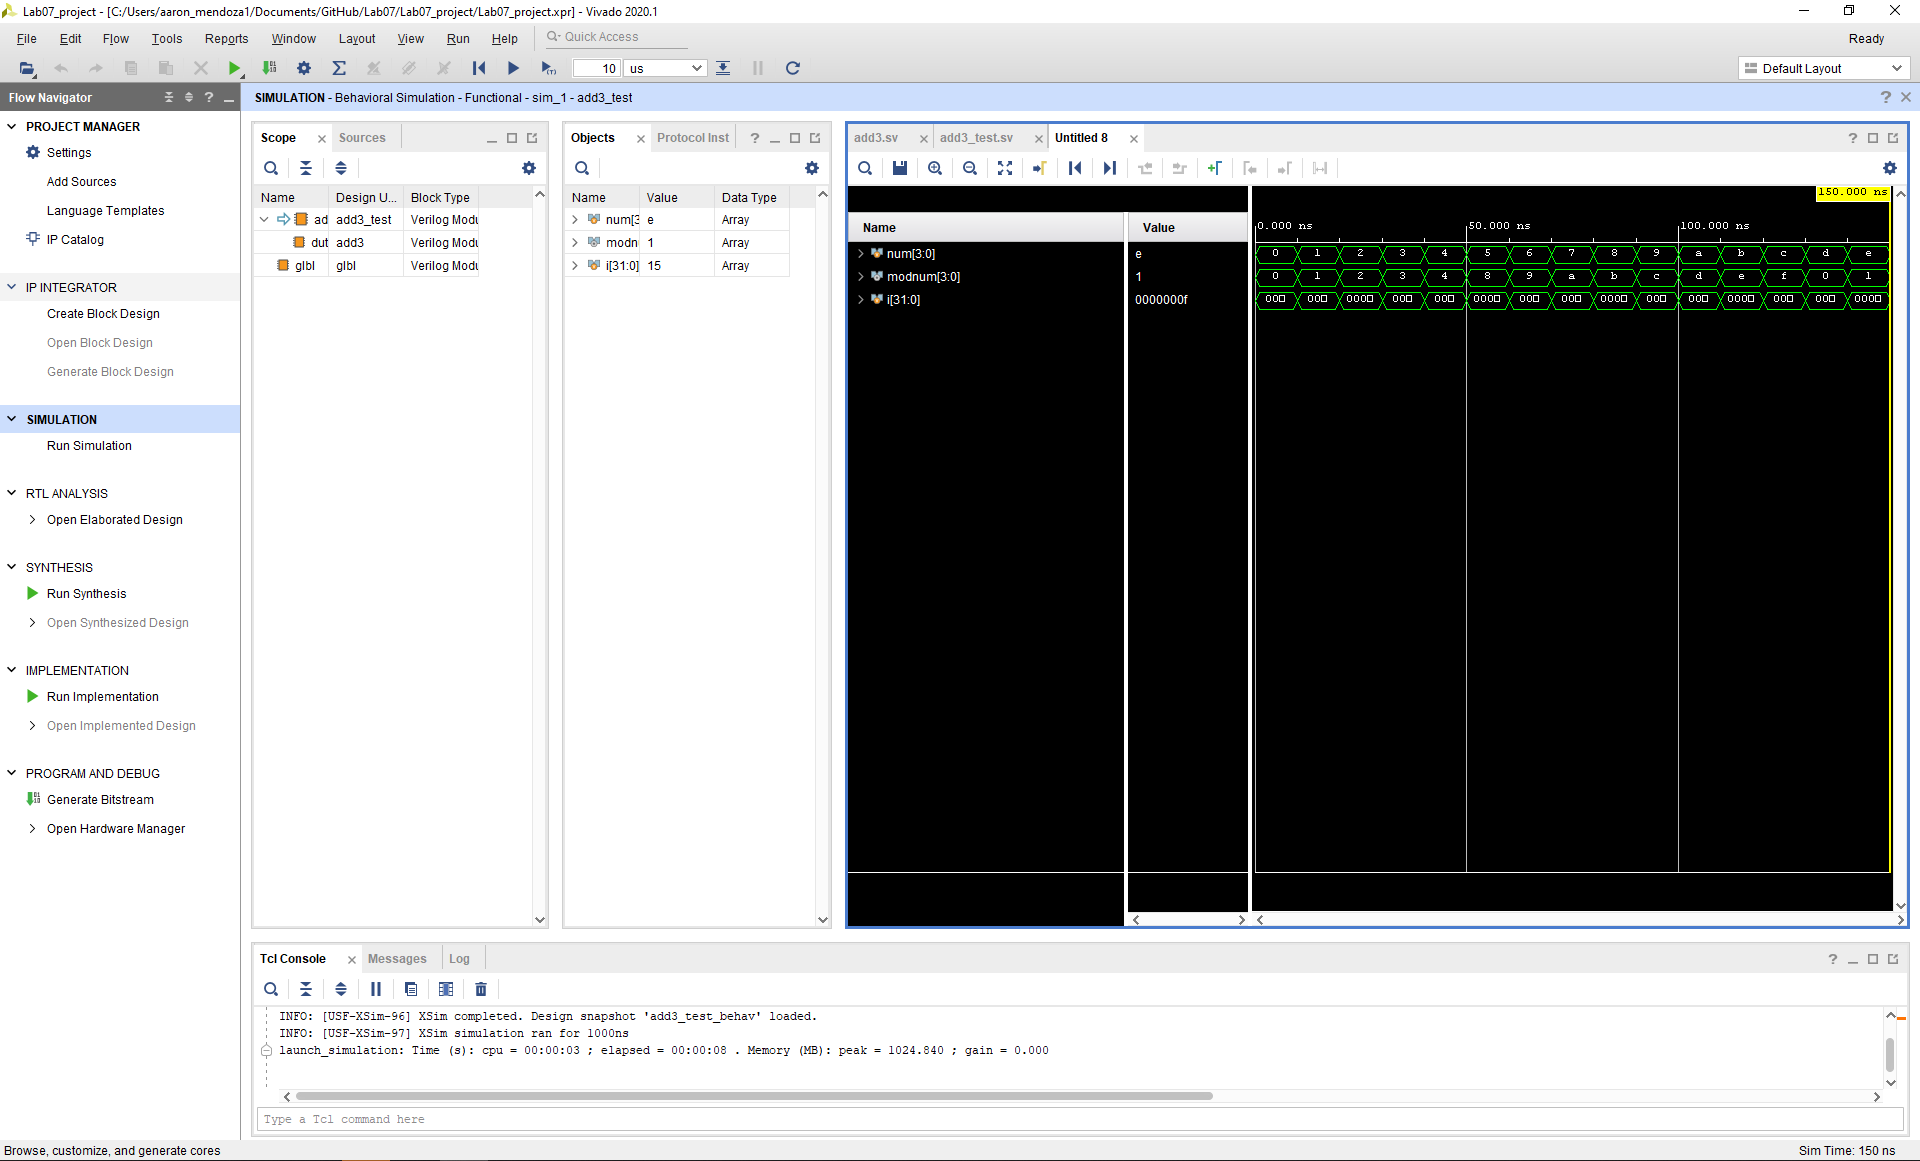
\includegraphics[width=1\textwidth,trim=19cm 15cm 0.5cm 4.5cm,clip]{add3_test_screenshot}
	\caption{Add 3 Module Simulation}
	\label{fig:sim_with_table}
\end{figure}

\begin{figure}[ht]\centering
	\caption{ERT for 6-Bit BCD Converter Module}
		\label{tbl:example_table}
		\begin{tabular}{c|cc}
			\toprule
			input & tens & ones \\
			\midrule
			000000 & 0000 & 0000 \\
			000001 & 0001 & 0001 \\
			000010 & 0000 & 0010 \\
			000011 & 0000 & 0011 \\
			000100 & 0000 & 0100 \\
			000101 & 0000 & 0101 \\
			........... & ....... & ........ \\
			111110 & 0110 & 0011 \\
			111111 & 0110 & 0100 \\
			\bottomrule
		\end{tabular} 
	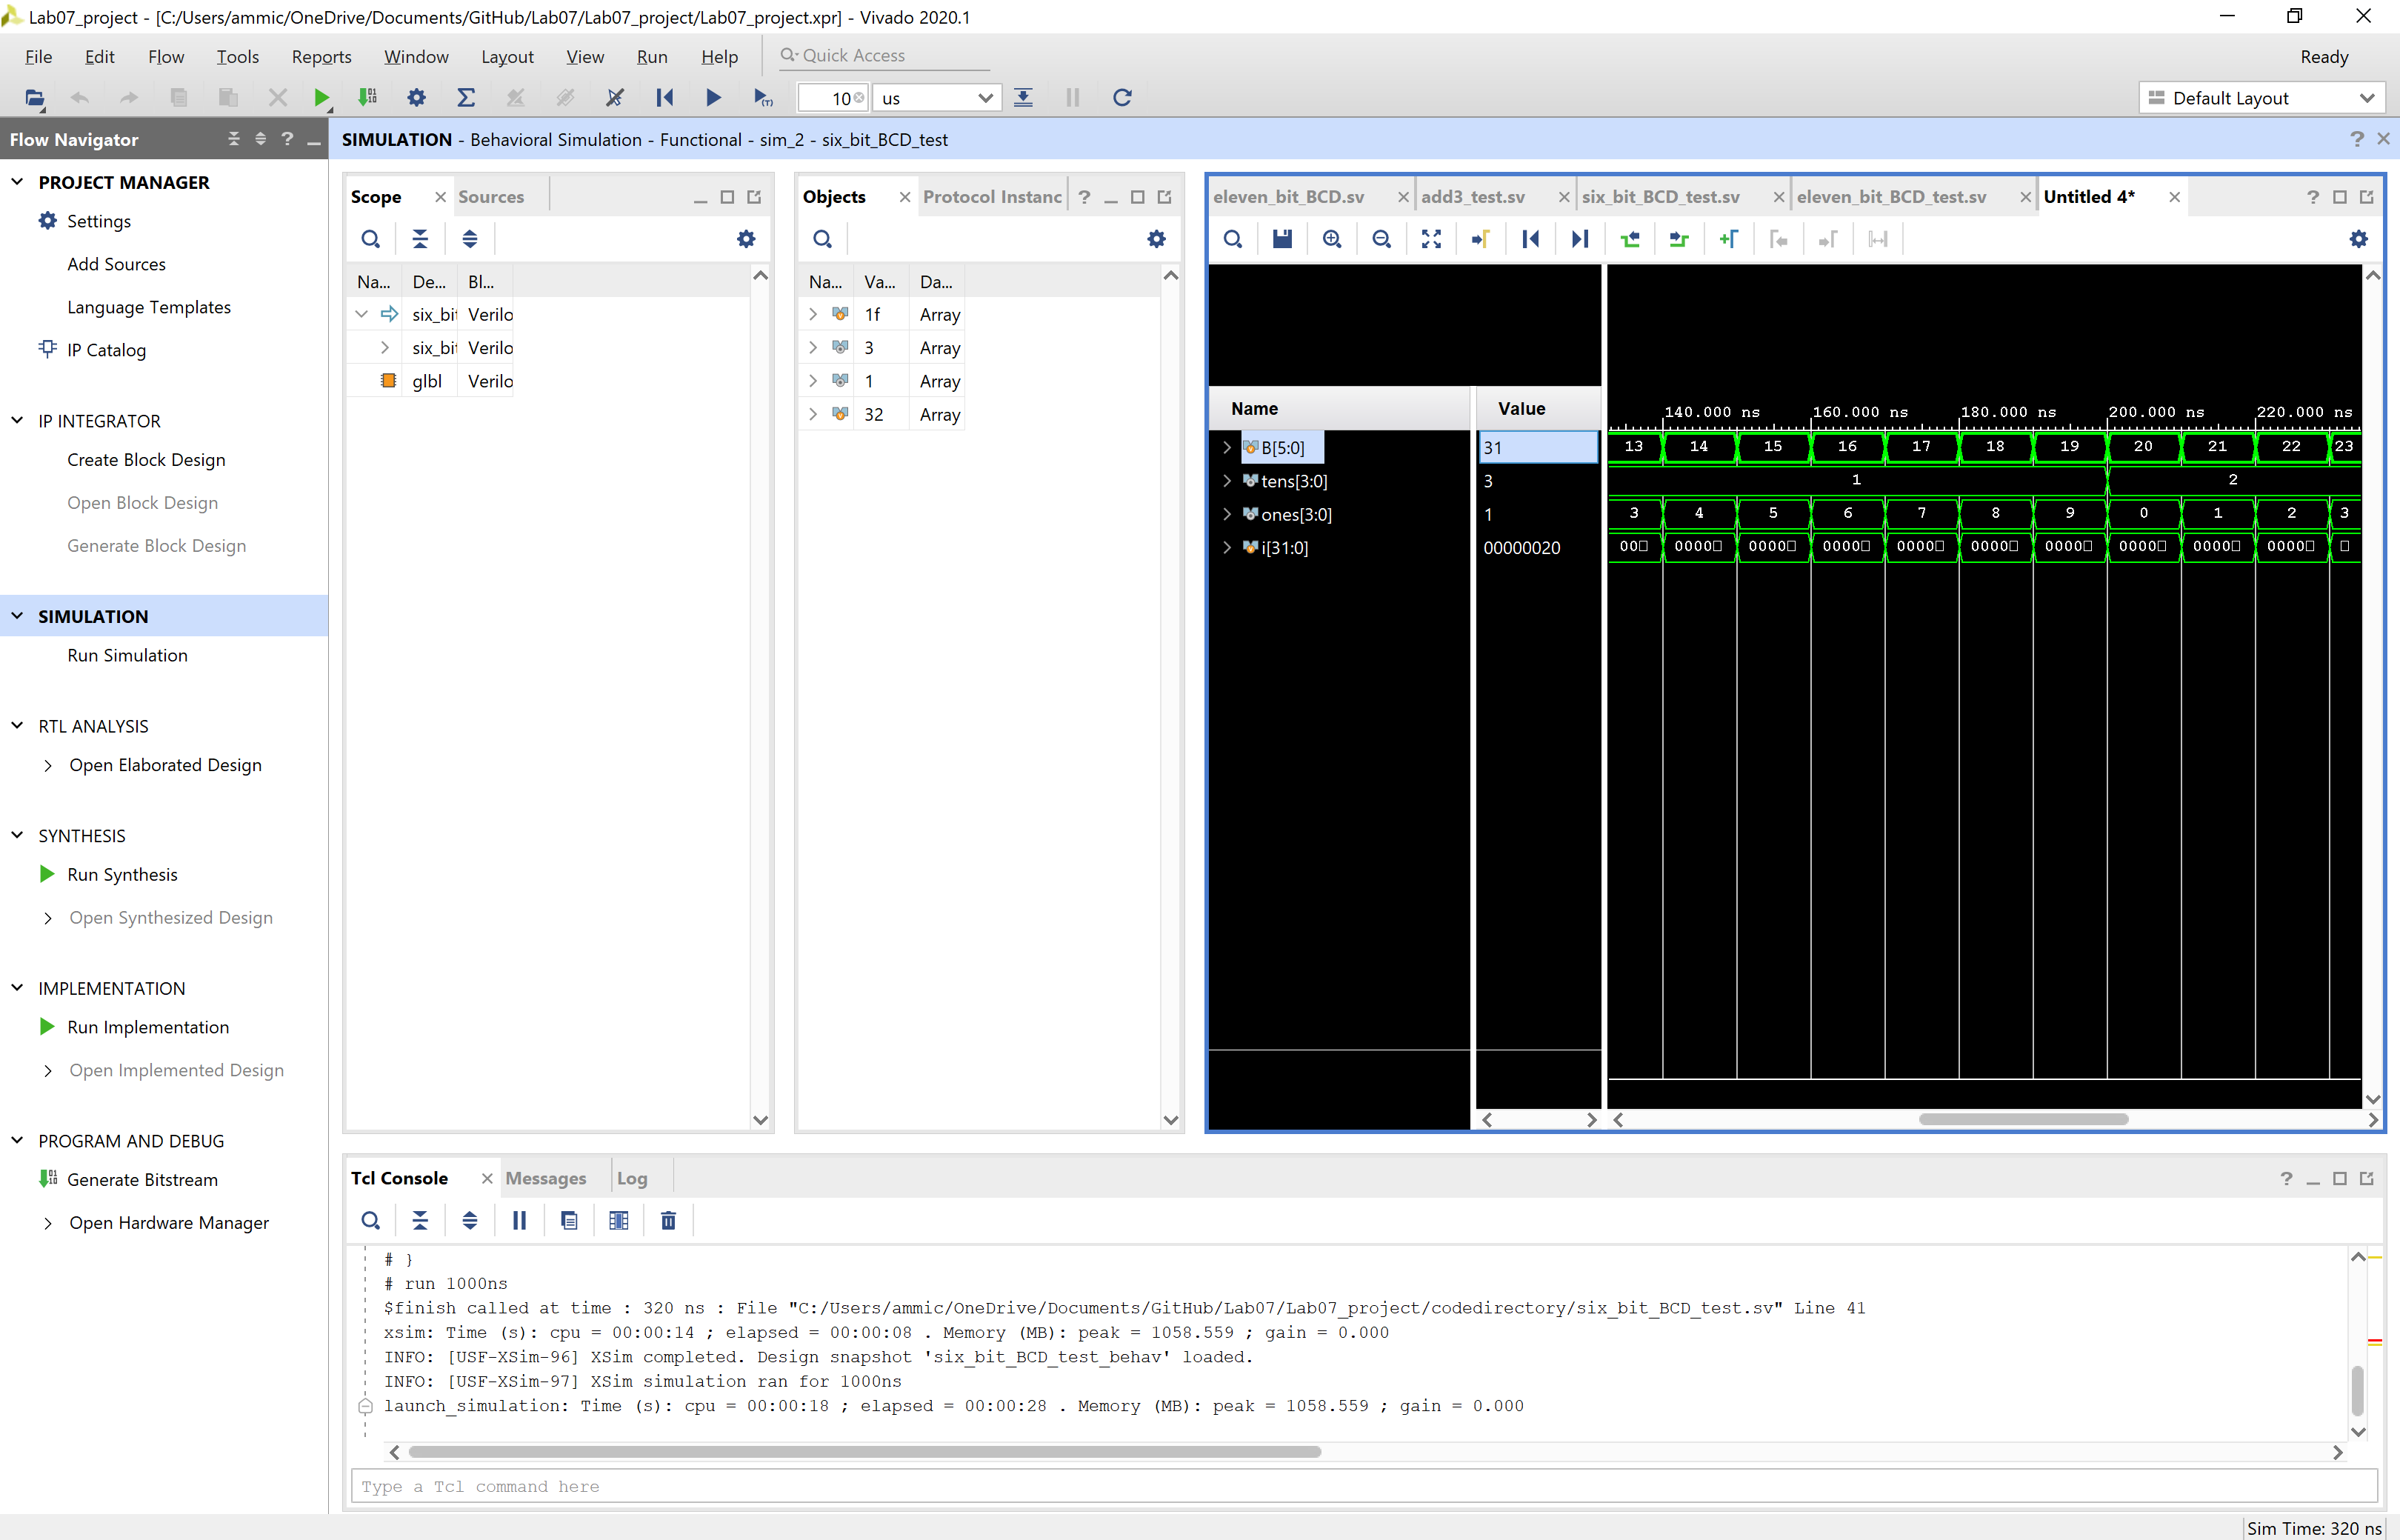
\includegraphics[width=1\textwidth,trim=19cm 15cm 0.5cm 4.5cm,clip]{six_BCD_test_screenshot}
	\caption{Six Bit Double-Dabble Module Simulation}
	\label{fig:sim_with_table}
\end{figure}

\begin{figure}[ht]\centering
	\caption{ERT for 11-Bit BCD Converter Module}
		\label{tbl:example_table}
		\begin{tabular}{c|cccc}
			\toprule
			input & thousands & hundreds & tens & ones \\
			\midrule
			00000000000 & 0000 & 0000 & 0000 & 0000 \\
			00000000001 & 0000 & 0000 & 0000 & 0001 \\
			00000000010 & 0000 & 0000 & 0000 & 0010 \\
			00000000011 & 0000 & 0000 & 0000 & 0011 \\
			.................... & ....... & ........ & ....... & ....... \\
			11111111110 & 0010 & 0000 & 0010 & 0111 \\
			11111111111 & 0010 & 0000 & 0010 & 1000 \\
			\bottomrule
		\end{tabular} 
	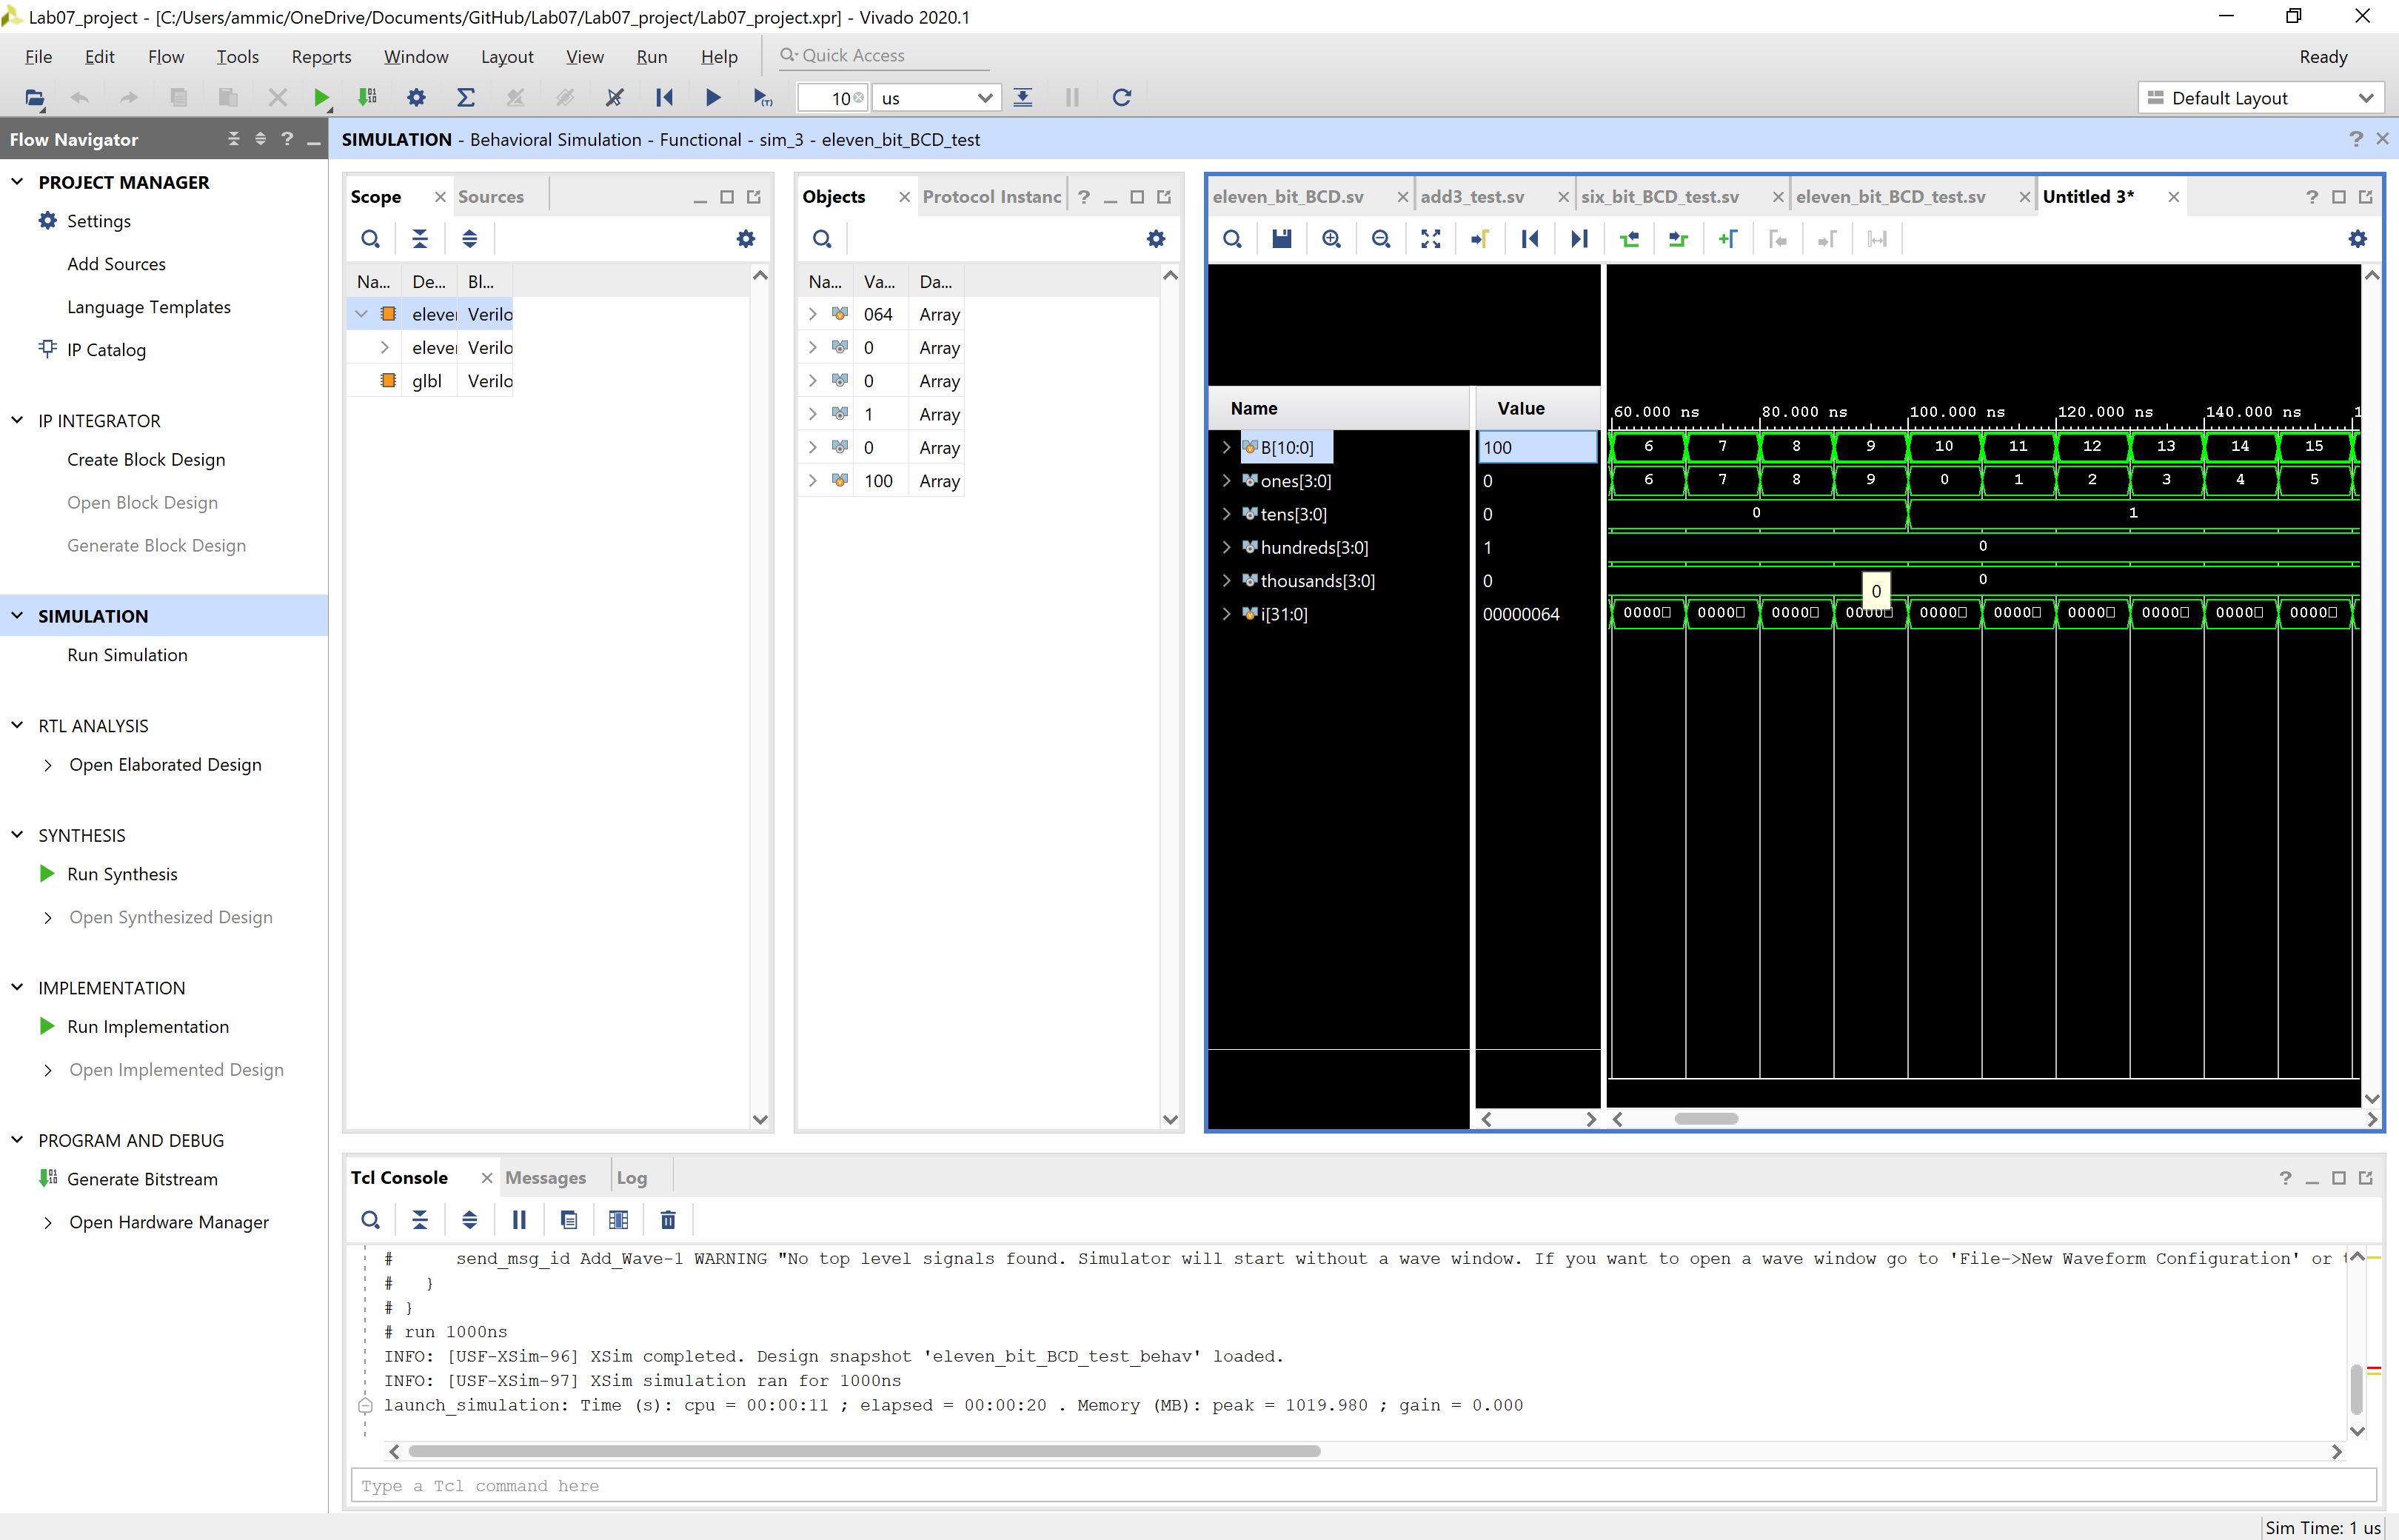
\includegraphics[width=1\textwidth,trim=19cm 15cm 0.5cm 4.5cm,clip]{elev_BCD_test_screenshot}
	\caption{Eleven Bit Double-Dabble Module Simulation}
	\label{fig:sim_with_table}
\end{figure}


\section*{Code}

\Verilog[firstline=22, lastline=40, caption=Add3 Module Code]{Lab07_project/codedirectory/add3.sv}|

\Verilog[firstline=22, lastline=42, caption=Add3 TB]{Lab07_project/codedirectory/add3_test.sv}|

\Verilog[firstline=22, lastline=50, caption=6-Bit BCD Converter Code]{Lab07_project/codedirectory/six_bit_BCD.sv}|

\Verilog[firstline=22, lastline=44, caption=6-Bit BCD Converter TB]{Lab07_project/codedirectory/six_bit_BCD_test.sv}|

\Verilog[firstline=22, lastline=114, caption=11-Bit BCD Converter Code]{Lab07_project/codedirectory/eleven_bit_BCD.sv}|

\Verilog[firstline=22, lastline=46, caption=11-Bit BCD Converter TB]{Lab07_project/codedirectory/elev_BCD_test_.sv}|

\Verilog[firstline=22, lastline=71, caption=Top Level Module]{Lab07_project/codedirectory/sseg1_BCD_wrapper.sv}|


\end{document}
